\chapter{Teoria da Integração}
\section{A Integral de Funções Não-Negativas}

Uma vez que já foram bem explorados os espaços mensuráveis e os espaços de medida, vamos medir funções mensuráveis de fato.
Iniciaremos por funções não negativas e iremos estendendo os conceitos aos poucos.
Quando não houver menção contrária, $(X, \Sigma, \mu)$ será um espaço de medida.
O conjunto de todas as funções $f:X \to \xreta$ mensuráveis será simplesmente denotado por $M = M(X, \Sigma)$ e o conjunto das funções não negativas, que também são $\Sigma$-mensuráveis será denotado por $M^+ = M^+(X, \Sigma)$. 
Assim, iniciaremos calculando a medida de funções simples

\begin{definition}[Função Simples]
    Uma função real é dita simples quando possui apenas uma quantidade finita de valores.
\end{definition}

Representaremos esse tipo de função, de forma padronizada em todo o texto, por meio da seguinte forma
$$
\varphi =  \sum_{j = 1}^n a_j\chi_{E_j}
$$
onde $a_j \in \R$ e $\chi_{E_j}$ é a função característica do conjunto $E_j \in \Sigma$.
Nessa representação estamos supondo que cada $a_j \in \R$ é diferente para todo $j \in \N$ e que
$\displaystyle \bigcup_{j = 1}^n E_j = X$.
As vezes, esse tipo de função também é chamado de função escada pelo formato de seu gráfico conforme veremos adiante.

\begin{example}
\label{ex:função-escada-part-1}
    Seja $f: [0,4] \to \R$ pondo $f(x) = 1$ se $x \in [0,2)$ e $f(x) = 2$ caso $x \in [2,4]$.
    Denotando $E_1 = [0,2), E_2 = [2,4], a_1 = 1$ e $a_2 = 2$ temos que
    $$
    f(x) = 1\cdot \chi_{[0,2)}(x) + 2\cdot \chi_{[2,4]}(x) = \sum_{j = 1}^2 a_j\chi_{E_j}(x)
    $$
    Além disso, $E_1 \cup E_2 = [0,2) \cup [2, 4] = [0,4]$ e $a_1 = 1\neq 2 = a_2$.
    Logo, $f$ é uma função simples. 
\end{example}

\begin{example}
\label{ex:função-escada-part-2}

    Seja $g: [0,4] \to \R$ pondo 
    
    $$g(x) = \left\{
    \begin{array}{cc}
         1, & \textrm{\ se } x \in [0,1] \\
         2, & \textrm{\ se } x \in (1,2] \\
         3, & \textrm{\ se } x \in (2,3] \\
         4, & \textrm{\ se } x \in (3,4]
    \end{array}\right.
    $$
    Claramente, $g$ também é uma função simples.
    Basta denotar $E_1 = [0,1), E_2 = (1,2], E_3 = (2,3], E_4 = (3,4]$ e $ a_i = i$ para $1 \leq i \leq 4$.
    Com isso, vemos que para $x \in [0,4]$
    $$
    g(x) = 1\cdot \chi_{[0,1]}(x) + 2\cdot \chi_{(1,2]}(x) + 3\cdot \chi_{(2,3]}(x) + 4\cdot \chi_{(3,4]}(x)
    $$
    Concluindo que $g = \dsum_{j = 1}^4 a_j\chi_{E_j}$. 
\end{example}
Note que os gráficos das funções $f$ e $g$ são, respectivamente.\\

    % Gráfico da função f
    \begin{figure}[h!]
	\centering
	\Caption{\label{fig:gráfico-função-simples-f-sobre-[0,4]} Gráfico da Função $f =\dsum_{j = 1}^2 a_j\chi_{E_j}$}	
	\UECEfig{}{
	    \begin{tikzpicture}[scale=0.55]
                % Eixos
                \draw[->] (-1,0) -- (5,0) node[right] {$x$};
                \draw[->] (0,-1) -- (0, 5) node[left] {$y$};
                                
                % Plot do gráfico
                \draw[domain=0:2,very thick,variable=\x,blue] plot ({\x},{1});
                \draw[domain=2:4,very thick,variable=\x,blue] plot ({\x},{2});
        
                % Bolinhas de intervalos aberto e fechado
                \draw[fill=white] (2,1) circle (0.08);
                \draw[fill=blue] (2,2) circle (0.08);

                % Rótulos
                \foreach \i in {-1,1,2,3,4}{
                \draw (\i,2pt)--(\i, -2pt) node[below]{{\footnotesize $\i$}};
                }
                
                \foreach \i in {-1,1,2,3,4}{
                \draw (2pt,\i)--(-2pt, \i) node[left]{{\footnotesize $\i$}};
                }
                % Linhas trastejadas
                % \draw[dashed, help lines] (2,0) -- (2,2);
                % \draw[dashed, help lines] (4,0) -- (4,2);
                
            \end{tikzpicture}
	}{
	    \Fonte{Elaborado pelo autor}
	}	
    \end{figure}    
    \begin{figure}[h!]
	\centering
	\Caption{\label{fig:gráfico-função-simples-f-sobre-[0,4]} Gráfico da Função $g =\dsum_{j = 1}^4 a_j\chi_{E_j}$}	
	\UECEfig{}{
	    \begin{tikzpicture}[scale=0.55]
                % Eixos
                \draw[->] (-1,0) -- (5,0) node[right] {$x$};
                \draw[->] (0,-1) -- (0, 5) node[left] {$y$};
                                
                % Plot do gráfico
                \draw[domain=0:1,very thick,variable=\x,blue] plot ({\x},{1});
                \draw[domain=1:2,very thick,variable=\x,blue] plot ({\x},{2});
                \draw[domain=2:3,very thick,variable=\x,blue] plot ({\x},{3});
                \draw[domain=3:4,very thick,variable=\x,blue] plot ({\x},{4});
        
                % Bolinhas de intervalos aberto e fechado
                \foreach \i in {1,2,3}{
                \draw[fill=white] (\i,\i+1) circle (0.08);
                }
                \foreach \i in {1,2,3,4}{
                \draw[fill=blue] (\i,\i) circle (0.08);
                }

                

                % Rótulos
                \foreach \i in {-1,1,2,3,4}{
                \draw (\i,2pt)--(\i, -2pt) node[below]{{\footnotesize $\i$}};
                }
                
                \foreach \i in {-1,1,2,3,4}{
                \draw (2pt,\i)--(-2pt, \i) node[left]{{\footnotesize $\i$}};
                }
                
                % Linhas trastejadas
                % \foreach \i in {1,2,3,4}{
                % \draw[dashed, help lines] (\i,0) -- (\i,\i);
                % }
                % \foreach \i in {1,2,3}{
                % \draw[dashed, help lines] (\i,\i) -- (\i,\i+1);
                % }  
            \end{tikzpicture}
	}{
	    \Fonte{Elaborado pelo autor}
	}	
    \end{figure} 
Agora pensemos na ideia de integral aprendida no cálculo integral.
Se quiséssemos calcular a integral das funções acima somaríamos as áreas dos retângulos conforme ilustram as figuras a seguir.\\
    % Integral da função f
    \begin{figure}[!h]
	\centering
	\Caption{\label{fig:integral-função-simples-f-sobre-[0,4]} Área delimitada pelo gráfico da função $f =\dsum_{j = 1}^2 a_j\chi_{E_j}$}	
	\UECEfig{}{
	    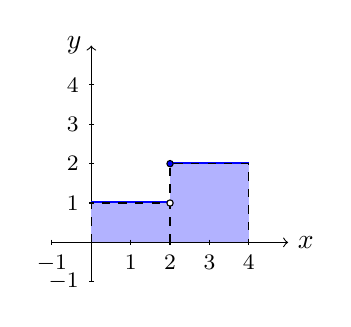
\begin{tikzpicture}[scale=0.5]
                % Eixos
                \draw[->] (-1,0) -- (5,0) node[right] {$x$};
                \draw[->] (0,-1) -- (0, 5) node[left] {$y$};
                                
                % Plot do gráfico
                \draw[domain=0:2,very thick,variable=\x,blue] plot ({\x},{1});
                \draw[domain=2:4,very thick,variable=\x,blue] plot ({\x},{2});
        
                
                % Retangulos

                \draw[fill=blue!30, dashed](0,0) rectangle (2,1);
                \draw[fill=blue!30, dashed](2,0) rectangle (4, 2);

                % Bolinhas de intervalos aberto e fechado
                \draw[fill=white] (2,1) circle (0.08);
                \draw[fill=blue] (2,2) circle (0.08);

                % Rótulos
                \foreach \i in {-1,1,2,3,4}{
                \draw (\i,2pt)--(\i, -2pt) node[below]{{\footnotesize $\i$}};
                }
                
                \foreach \i in {-1,1,2,3,4}{
                \draw (2pt,\i)--(-2pt, \i) node[left]{{\footnotesize $\i$}};
                }
                % Linhas trastejadas
                % \draw[dashed, help lines] (2,0) -- (2,2);
                % \draw[dashed, help lines] (4,0) -- (4,2);
                
            \end{tikzpicture}
	}{
	    \Fonte{Elaborado pelo autor}
	}	
    \end{figure}
    \\
    %Gráfico da função g
    \begin{figure}[!h]
	\centering
	\Caption{\label{fig:integral-função-simples-f-sobre-[0,4]} Área delimitada pelo gráfico da função $g =\dsum_{j = 1}^4 a_j\chi_{E_j}$}	
	\UECEfig{}{
	    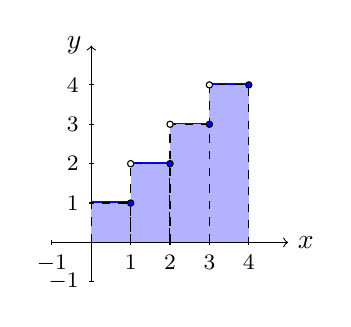
\begin{tikzpicture}[scale=0.5]
                % Eixos
                \draw[->] (-1,0) -- (5,0) node[right] {$x$};
                \draw[->] (0,-1) -- (0, 5) node[left] {$y$};
                                
                % Plot do gráfico
                \draw[domain=0:1,very thick,variable=\x,blue] plot ({\x},{1});
                \draw[domain=1:2,very thick,variable=\x,blue] plot ({\x},{2});
                \draw[domain=2:3,very thick,variable=\x,blue] plot ({\x},{3});
                \draw[domain=3:4,very thick,variable=\x,blue] plot ({\x},{4});

                % Retangulos
                \foreach \i in {0, 1,2,3}{
                \draw[fill=blue!30, dashed](\i,0) rectangle (\i+1,\i +1);
                }
                
                % Bolinhas de intervalos aberto e fechado
                \foreach \i in {1,2,3}{
                \draw[fill=white] (\i,\i+1) circle (0.08);
                }
                \foreach \i in {1,2,3,4}{
                \draw[fill=blue] (\i,\i) circle (0.08);
                }

                % Rótulos
                \foreach \i in {-1,1,2,3,4}{
                \draw (\i,2pt)--(\i, -2pt) node[below]{{\footnotesize $\i$}};
                }
                
                \foreach \i in {-1,1,2,3,4}{
                \draw (2pt,\i)--(-2pt, \i) node[left]{{\footnotesize $\i$}};
                }
                
                % Linhas trastejadas
                % \foreach \i in {1,2,3,4}{
                % \draw[dashed, help lines] (\i,0) -- (\i,\i);
                % }
                % \foreach \i in {1,2,3}{
                % \draw[dashed, help lines] (\i,\i) -- (\i,\i+1);
                % }  
            \end{tikzpicture}
	}{
	    \Fonte{Elaborado pelo autor}
	}	
    \end{figure} 

\begin{definition}
\label{def:integral-função-naonegativa-simples}
    Se $\varphi$ é uma função simples de $M^+(X, \Sigma)$ com a representação apresentada anteriormente, então a integral da função $\varphi$ com respeito à medida $\mu$ é o valor real estendido
    $$
    \int\varphi d\mu = \sum_{j = 1}^n a_j\mu(E_j).
    $$
\end{definition}

Para a definição \ref{def:integral-função-naonegativa-simples} empregamos a convenção que $0 \cdot (+\infty) = 0$.
Isto é feito para garantir que a função identicamente nula tenha integral nula independentemente da medida ser finita ou não.
Veremos propriedades elementares sobre a integral de funções simples, mas antes provaremos alguns resultados auxiliares.

\begin{lemma}
\label{lem:medida-da-intersecao-de-um-fixado}
    Se $\mu$ é uma medida sobre $X$ e fixemos um elemento $A$ de $\mathcal{H}$, então a função $\lambda$ definida por $\lambda(E) = \mu(A\cap E), \ \forall E \in \h$ é uma medida sobre $X$.
\end{lemma}
\begin{prova}
    Basta mostrar que $\lambda$ satisfaz as condições impostas na definição \ref{def:medida}.
    Com isso, se $E = \varnothing$, então
    $$
    \lambda(\varnothing) = \mu(A \cap \varnothing) = \mu(\varnothing) = 0
    $$
    Como $A$ e $E$ são elementos de $\h$, então $A \cap H$ também está em $\h$.
    Assim, por $\mu$ ser uma medida, temos que $\mu(A\cap E) \geq 0$ acarretando que $\lambda(E) \geq 0$.
    Por fim, tomemos uma sequência de elementos disjuntos $(E_n)$ em $\h$.
    Se $A = E_j$ para algum $j \in \N$, não há o que fazer.
    Caso $A \cap E_j = \varnothing$ para qualquer que seja $j \in \N$, então $\displaystyle \left( \bigcup_{n \in \N} E_n\right) \cap A = \varnothing$.
    Com isso, 

    \begin{align*}
        \left( \bigcup_{n \in \N} E_n\right) \cap A
        = &
        (E_1 \cup E_2 \cup \cdots \cup E_n \cup \cdots) \cap A\\
        = &
        (E_1 \cap A )\cup (E_2 \cap A) \cup \cdots \cup (E_n\cap A) \cup \cdots \\
        = &
        \bigcup_{n \in \N} (E_n\cap A)    
    \end{align*}
    %   
    Segue então que
    $$
    \lambda\left( \bigcup_{n \in \N} E_n\right)
    =
    \mu\left(\left( \bigcup_{n \in \N} E_n\right) \cap A\right)
    =
    \mu\left( \bigcup_{n \in \N} (E_n\cap A) \right)
    =
    \sum_{j = 1}^\infty \mu(E_j \cap A)
    = 
    \sum_{j = 1}^\infty \lambda(E_j)
    $$
    Com isso, concluímos que a função $\lambda$ acima definida é uma medida.
\end{prova}

\begin{lemma}
\label{lem:medida-gerada-por-medidas-e-numeros-reais}
    Se $\mu_1, ..., \mu_n$ são medidas sobre $X$ e $a_1, ... , a_n$ são números reais não negativos, então a função $\lambda$ definida por
    $\lambda(E) = \dsum_{j =1}^n a_j\mu_j(E), \forall E \in \Sigma$ é uma medida sobre $X$.
\end{lemma}
\begin{prova}
    Como $\mu_j$ é uma medida para todo $j \in I_n$ e cada $a_j$ é maior ou igual à zero, temos que cada $a_j\mu_j(E) \geq 0$.
    Desta forma, $\lambda(E) = \displaystyle \sum_{j = 1}^n a_j\mu_j(E) \geq 0$.
    Além disso, podemos observar que $\lambda(\varnothing) = \displaystyle \sum_{j =1}^n a_j\mu_j(\varnothing) = 0$.
    Tomemos uma sequência disjunta $(E_p)$ de elementos de $\h$.
    Logo, 
    $$
    \lambda\left(\bigcup_{p \in \N} E_p\right)
    =
    \sum_{j = 1}^n a_j\mu_j\left(\bigcup_{p \in \N} E_p\right)
    =
    \sum_{j = 1}^n a_j\left(\sum_{p = 1}^\infty\mu_j(E_p)\right)
    $$
    Afirmamos que $\displaystyle \sum_{j = 1}^n a_j\left(\sum_{p = 1}^\infty\mu_j(E_p)\right) = \sum_{p = 1}^\infty\left(\sum_{j = 1}^na_j\mu_j(E_p)\right)$.
    Com efeito, 
    \begin{align*}
        \sum_{j = 1}^n a_j\left(\sum_{p = 1}^\infty\mu_j(E_p)\right)
        = &
        \sum_{j = 1}^n a_j\left(\lim_{m \to +\infty}\sum_{p = 1}^m\mu_j(E_p)\right)\\
        = &
        \lim_{m \to +\infty}\left[\sum_{j = 1}^n a_j\left(\sum_{p = 1}^m\mu_j(E_p)\right)\right]\\
        = &
        \lim_{m \to +\infty}\left[a_1\left(\sum_{p = 1}^m\mu_1(E_p)\right)+ \cdots + a_n\left(\sum_{p = 1}^m\mu_n(E_p)\right)\right]\\
        = &
        \lim_{m \to +\infty}\left(\sum_{p = 1}^ma_1\mu_1(E_p)+ \cdots + \sum_{p = 1}^ma_n\mu_n(E_p)\right)\\
        = &
        \lim_{m \to +\infty}\sum_{p = 1}^m \left(a_1\mu_1(E_p)+ \cdots + a_n\mu_n(E_p)\right)\\
        = &
        \lim_{m \to +\infty}\sum_{p = 1}^m \left(\sum_{j = 1}^na_j\mu_j(E_p)\right)\\
        = &
        \sum_{p = 1}^\infty \left(\sum_{j = 1}^na_j\mu_j(E_p)\right)\\
    \end{align*}
    Disso tudo, obtemos que 
    $$
    \lambda\left(\bigcup_{p \in \N} E_p\right)
    =
    \sum_{j = 1}^n a_j\left(\sum_{p = 1}^\infty\mu_j(E_p)\right)
    =
    \sum_{p = 1}^\infty \left(\sum_{j = 1}^na_j\mu_j(E_p)\right)
    =
    \sum_{p = 1}^\infty \lambda(E_p)
    $$
    Como $\lambda$ satisfaz todas as condições impostas na definição \ref{def:medida} concluímos que $\lambda$ é uma medida.    
\end{prova}




\begin{theorem}
    Se $\varphi$ e $\psi$ são funções simples do espaço $M^+(X,\Sigma)$ e $c\geq0$ é uma constante real, então
    $$
    \int c\varphi d\mu = c \int \varphi d\mu,
    $$
    $$
    \int (\varphi + \psi) d\mu = \int \varphi d\mu + \int \psi d\mu.
    $$
\end{theorem}
\begin{prova}
    Vamos representar as funções simples não negativas por $\varphi = \dsum_{j = 1}^n a_j\chi_{E_j}$ e $\psi = \dsum_{k = 1}^m a_k\chi_{F_k}$.
    Caso $c = 0$, o resultado é verdadeiro trivialmente. 
    Supondo $c> 0$, temos que
    $$\int c \varphi\ d\mu = \dsum_{j = 1}^n c a_j\mu(E_j) = c \dsum_{j = 1}^n a_j\mu(E_j) = c\int \varphi \ d\mu.$$
    Dadas as representações padrão de $\varphi$ e $\psi$, vemos que $\varphi +\psi$ tem a representação 
    $$
    \varphi + \psi = \dsum_{j = 1}^n\dsum_{k = 1}^m(a_j + b_k)\chi_{E_j \cap F_k}.
    $$
    Entretanto, essa representação não é, necessariamente, a representação padrão apresentada na definição \ref{def:integral-função-naonegativa-simples}, pois 
    nada garante, previamente, que $a_j + b_k$ sejam distintos para $j \in I_n$ e $k \in I_m$.
    Com isso, sejam $c_h$, com $h \in I_p$, números distintos do conjunto $\{a_j + b_k; \ (j,k) \in I_n \times I_m\}$ e $G_h$ a união de todos os conjuntos $E_j \cap F_k \neq \varnothing$ tal que $a_j + b_k = c_h$.
    Assim, 
    $$
    G_h = \bigcup_{\begin{minipage}{1.4cm}
        \fontsize{8}{5}\selectfont
        \centering
        $j,k$
        $a_j + b_k = c_h$
    \end{minipage}} E_j \cap F_k
    $$
    A notação utilizada acima indica que a soma é realizada sobre todos os índices $j$ e $k$ tais que $a_j + b_k =c_h$.
    Como $E_j \cap F_k = \varnothing$, temos que 
    $$
    \mu(G_h) = \mu\left(\bigcup_{
        j,k\atop
        a_j + b_k = c_h} E_j \cap F_k
    \right)
    = 
    \sum_{
        j,k\atop
        a_j + b_k = c_h} \mu(E_j \cap F_k)
    $$
    Desta forma, conseguimos encontrar uma representação padrão que é dada por 
    $\displaystyle \varphi + \psi = \sum_{h =1}^p c_h\chi_{G_h}$.
    Logo, temos que 
    \begin{align*}
        \int(\varphi + \psi) d\mu = \sum_{h =1}^p c_h\mu(G_h)
        = & 
        \sum_{h = 1}^p\sum_{ j,k\atop a_j + b_k = c_h}c_h \mu(E_j \cap F_k)\\
        = &
        \sum_{h = 1}^p\sum_{ j,k\atop a_j + b_k = c_h}(a_j + b_k) \mu(E_j \cap F_k)\\
        = &
        \sum_{j = 1}^n\sum_{k = 1}^m(a_j + b_k) \mu(E_j \cap F_k)\\
        = &
        \sum_{j = 1}^n\sum_{k = 1}^m a_j \mu(E_j \cap F_k) + \sum_{j = 1}^n\sum_{k = 1}^m b_k \mu(E_j \cap F_k)
    \end{align*}
    Ora, uma vez que $X$ é a união de ambas as famílias disjuntas $\{E_j\}$ e $\{F_k\}$, isto é, 
    $$
    \bigcup_{j = 1}^n E_j = X = \bigcup_{k = 1}^m F_k 
    $$
    Desta forma, se um elemento $x$ pertence à um conjunto $E_{j_0}$ para algum $j_0 \in I_n$, então deve existir um $k_0 \in I_m$ tal que $x \in F_{k_0}$.
    Assim, se fixamos um $j \in I_n$, então $\bigcup_{k \in I_m} F_k$ forma uma cobertura de $E_j$, isto é, 
    $\displaystyle E_j \subset \bigcup_{k \in I_m} F_k$.
    Assim, 
    $\displaystyle E_j \cap \left(\bigcup_{k \in I_m} F_k\right) = E_j$. Como ${F_k}$ é uma família disjunta segue que, para este $j$ fixado, temos
    $$
    \mu(E_j) = \mu\left(E_j \cap \bigcup_{k \in I_m} F_k\right)
    = \mu\left(\bigcup_{k \in I_m} (E_j \cap F_k)\right)
    = \sum_{k = 1}^m \mu(E_j \cap F_k)
    $$
    Analogamente, ao fixarmos um $k \in I_m$, vemos que $\displaystyle \mu(F_k) = \sum_{j = 1}^n \mu(E_j \cap F_k)$.
    Empregando este resultado ao que foi desenvolvido anteriormente obtemos
    $$
    \sum_{j = 1}^n\sum_{k = 1}^m a_j \mu(E_j \cap F_k) + \sum_{j = 1}^n\sum_{k = 1}^m b_k \mu(E_j \cap F_k)
    =
    \sum_{j = 1}^n a_j \mu(E_j) + \sum_{k = 1}^m b_k \mu(F_k)
    =
    \int \varphi d\mu + \int \psi d\mu
    $$
    Segue que $\displaystyle\int(\varphi + \psi) d\mu = \int \varphi d\mu + \int \psi d\mu$ como queríamos.
\end{prova}
